\documentclass[12pt,a4paper,titlepage,oneside]{report}
\usepackage[utf8]{inputenc}
\usepackage[T1]{fontenc}
\usepackage[french]{babel}
\usepackage[top=1.5cm, bottom=5cm]{geometry}
\usepackage{fancyhdr, graphicx, array, pdfpages}
\usepackage[breaklinks]{hyperref}

\pagestyle{fancy}

\title{\textsc{\textbf{ Dossier
            \\Interpréteur du langage LIR}
}}
\date{}
\author{Nicolas \textsc{Caminade} \and Sylvan \textsc{Courtiol} \and Pierre
    \textsc{Debas} \and Heïa \textsc{Dexter} \and Lucàs \textsc{Vabre} }

\begin{document}

    % En-tête et pied de page ........................................
    \lhead{\leftmark}
    \rhead{
        
\includegraphics[width=2cm]{img/logoiut}
    }

    \cfoot{\thepage}
    \headheight = 2cm
    \headsep = 1.5cm

    % Page de garde ..................................................
    \begin{titlepage}
        \fontfamily{pag}\selectfont

        \begin{center}\normalsize
            \MakeUppercase{IUT de Rodez \hfill Département informatique
                \hfill INFO1 2020-2021}
        \end{center}
        \vspace*{0.1cm}
        \hrule
        \vspace*{0.2cm}
        \begin{flushright}
            
\includegraphics[width=4cm]{img/logoiut}
        \end{flushright}
        \vspace*{2cm}
        \begin{flushright}\Huge
            \textsc{\textbf{ Dossier
                    \\Interpréteur du langage LIR}}
        \end{flushright}
        \hrule
        \begin{flushleft}
            \MakeUppercase{Projet proposé par Frédérique Barrios}
        \end{flushleft}
        \vspace*{2cm}
        \begin{center}\Large
            Nicolas \textsc{Caminade}, Sylvan \textsc{Courtiol},\\
            Pierre \textsc{Debas}, Heïa \textsc{Dexter}, \\
            Lucàs \textsc{Vabre}
        \end{center}
        \vfill
        \begin{center}\normalsize
            \MakeUppercase{Projet tuteuré --- Semestre 2}
        \end{center}
    \end{titlepage}

    \renewcommand{\contentsname}{Sommaire}
    \tableofcontents

    % Fin de votre introduction ......................................

    \normalsize
    % Début du corps de votre document ...............................
    \addcontentsline{toc}{part}{Sommaire}
    \part{Plan projet\\(annexe)}
%    \setcounter{chapter}{0}
    \part{ Spécifications détaillées}
%    \setcounter{chapter}{0}
    \documentclass[12pt,a4paper,titlepage,openany, oneside]{report}
\usepackage[utf8]{inputenc}
\usepackage[T1]{fontenc}
\usepackage[french]{babel}
\usepackage[top=1.5cm, bottom=4cm]{geometry}
\usepackage{fancyhdr, graphicx, array, hyperref}

\pagestyle{fancy}

\title{\textsc{\textbf{Spécifications détaillées\\Interpréteur du langage LIR}}}
\date{}
\author{Nicolas \textsc{Caminade} \and Sylvan \textsc{Courtiol} \and
    Pierre \textsc{Debas} \and Heïa \textsc{Dexter} \and Lucàs
    \textsc{Vabre} }
\begin{document}
    \lhead{\leftmark}
    \rhead{
        
\includegraphics[width=2cm]{./img/logoiut}
    }

    \cfoot{\thepage}
    \headheight = 2cm
    \headsep = 0.5cm

    \begin{titlepage}
        \fontfamily{pag}\selectfont

        \begin{center}\normalsize
            \MakeUppercase{IUT de Rodez \hfill Département informatique
                \hfill INFO1 2020-2021}
        \end{center}
        \vspace*{0.1cm}
        \hrule
        \vspace*{0.2cm}
        \begin{flushright}
            
\includegraphics[width=4cm]{./img/logoiut}
        \end{flushright}
        \vspace*{2cm}
        \begin{flushright}\Huge
            \textsc{\textbf{Spécifications détaillées
                    \\Interpréteur du langage LIR}}
        \end{flushright}
        \hrule
        \begin{flushleft}
            \MakeUppercase{Projet proposé par Frédérique Barrios}
        \end{flushleft}
        \vspace*{2cm}
        \begin{center}\Large
            Nicolas \textsc{Caminade}, Sylvan \textsc{Courtiol},\\
            Pierre \textsc{Debas}, Heïa \textsc{Dexter}, \\
            Lucàs \textsc{Vabre}
        \end{center}
        \vfill
        \begin{center}\normalsize
            \MakeUppercase{Projet tuteuré --- Semestre 2}
        \end{center}
    \end{titlepage}

    \renewcommand\rmdefault{pag}
    \fontfamily{pag}\selectfont
    \renewcommand{\sfdefault}{pag}

    % Sommaire
    \renewcommand{\contentsname}{Sommaire}
    \tableofcontents

    \chapter*{Introduction}
    \Large
    Texte. Blablabla

    \footnotesize
    \chapter{Récits d'utilisation proposés lors de l'itération 1}
        \section{Commande}

    \subsection*{Récit d'utilisation}

    \paragraph{Titre : } Exécution d'une commande
        \paragraph{Récit : } Exécution d'une commande
    \paragraph{En tant que : } programmeur avec l'interpréteur LIR
    \paragraph{Je souhaite : } exécuter une commande
    \paragraph{Afin de : } obtenir le résultat de cette commande ou une
                               confirmation de son exécution
    \subsection*{Critères d'acceptation}

    \paragraph{À partir du fait : } l'interpréteur affiche un invite
    \paragraph{Alors : } j'entre une ligne de commande
    \paragraph{Enfin : } j'obtiens le résultat de cette commande ou un retour
    m'informant du bon déroulé de l'exécution de la commande ou de son échec.
    \newpage
        \section{Commande debut}
    \subsection*{Récit d'utilisation}

    \paragraph{Titre : } debut
    \paragraph{Récit : } Réinitialiser l'environnement de l'interpréteur LIR
    \paragraph{En tant que : } programmeur
    \paragraph{Je souhaite : } vider l'intégralité du contexte d'exécution
    \paragraph{Afin de : } obtenir un environnement de travail vierge

    \subsection*{Critères d'acceptation}

    \paragraph{À partir de : } d'une session de l'interpréteur LIR
    \paragraph{Alors : } j'entre la commande \verb|debut|
    \paragraph{Enfin : } L'interpréteur efface toutes les lignes de programme
    mémorisées ainsi que tous les identificateurs mémorisés
        \section{Commande fin}

    \subsection*{Récit d'utilisation}

    \paragraph{Titre : } Quitter l'interpréteur (commande fin)
    \paragraph{Récit : } Quitter l'interpréteur (commande fin)
    \paragraph{En tant que : } programmeur avec l'interpréteur LIR
    \paragraph{Je souhaite : } quitter l'interpréteur
    \paragraph{Afin de : } arrêter d'utiliser l'interpréteur LIR pour la session courante

    \subsection*{Critères d'acceptation}

    \paragraph{À partir du fait : } je suis en train d'utiliser l'interpréteur
    \paragraph{Alors : } je souhaite quitter l'interpréteur pour la session courante en exécutant la commande fin
    \paragraph{Enfin : } le processus courant de l'interpréteur LIR s'arrête
        \section{Commande defs}
    \subsection*{Récit d'utilisation}

    \paragraph{Titre : } Affichages du contexte courant (commande defs) % Écrire le titre à la place du commentaire
    \paragraph{Récit : } Affichages du contexte courant (commande defs) % Écrire nom du récit à la suite
    \paragraph{En tant que : } programmeur avec l'interpréteur LIR % Remplacer commentaire par rôle
    \paragraph{Je souhaite : } voir toutes les variables définies dans la session courante (identificateur et valeur)
    \paragraph{Afin de : } connaître le contexte actuel de la session courante de l'interpréteur

    \subsection*{Critères d'acceptation}

    \paragraph{À partir du fait : } des variables sont définies dans la session courante de l'interpréteur
    \paragraph{Alors : } je souhaite connaître le contexte actuel en exécutant la commande defs
    \paragraph{Enfin : } l'interpréteur affiche chaque variable ligne par ligne avec son identificateur et sa valeur

        \section{Commande affiche}

	\subsection*{Récit d'utilisation}

	\paragraph{Titre : } Faire un saut de ligne avec la commande affiche
	\paragraph{Récit : }  Provoquer le saut de ligne sur la sortie de texte courante
	\paragraph{En tant que : } Programmeur
	\paragraph{Je souhaite : } que l'interpréteur LIR saute une ligne sur la sortie de texte courante
	\paragraph{Afin de : } Provoquer un saut de ligne sur cette sortie

	\subsection*{Critères d'acceptation}

	\paragraph{À partir du fait : } que j'ai une sortie de texte courante
	\paragraph{Alors : } j'entre la commande affiche
	\paragraph{Enfin : } l'interpréteur saute une ligne sur la sortie de texte courante
        \section{Commande affiche avec une expression}

	\subsection*{Récit d'utilisation}

	\paragraph{Titre : } Commande affiche (expression)
	\paragraph{Récit : }  Afficher le contenu d'une expression sur la console de l'interpréteur
	\paragraph{En tant que : } Programmeur
	\paragraph{Je souhaite : } que l'interpréteur LIR évalue et affiche le contenu de l'expression que l'on lui donne
	\paragraph{Afin de : } pouvoir récupérer/vérifier le/les résultat(s) de son programme

	\subsection*{Critères d'acceptation}

	\paragraph{À partir du fait : } que j'ai la possibilité de saisir une ligne de commande
	\paragraph{Alors : } je tape la commande affiche et écrit l'expression dont je veut que la valeur soit affichée à la suite : affiche <expression>
	\paragraph{Enfin : } l'interpréteur évalue dans l'expression spécifiée la valeur de celle-ci et renvoie cette valeur sur la console et affiche un résultat sur LIR (en tant que feed-back) pour nous spécifier si la commande a bien pu s'exécuter

        \section{Commande var pour une chaîne de caractères}

    \subsection*{Récit d'utilisation}

    \paragraph{Titre : } Commande var (Chaine de caractères)
    \paragraph{Récit : }  Initialiser une chaine de caractère dans variable / Changer sa valeur
    \paragraph{En tant que : } Programmeur
    \paragraph{Je souhaite : } que l'interpréteur LIR stock une chaine dans une variable
    \paragraph{Afin de : } pouvoir récupérer/manipuler cette chaine plus tard dans le programme


    \subsection*{Critères d'acceptation}

    \paragraph{À partir du fait : } que j'ai la possibilité de saisir une ligne de commande
    \paragraph{Alors : } je tape la commande var et met une chaine de caractère entre double guillements comme valeur : var <nomVariable>="<chaine>"
    \paragraph{Enfin : } l'interpréteur enregistre dans la variable spécifié la chaine de caractère voulue et renvoie la variable suivie de sa valeur (en tant que feed-back)
        \section{Commande var pour un entier}
   \subsection*{Récit d'utilisation}

    \paragraph{Titre : } Commande var (Entier)
    \paragraph{Récit : }  Initialiser un entier dans variable / Changer sa valeur
    \paragraph{En tant que : } Programmeur
    \paragraph{Je souhaite : } que l'interpréteur LIR stock un entier dans une variable
    \paragraph{Afin de : } pouvoir récupérer/manipuler cet entier plus tard dans le programme

    \subsection*{Critères d'acceptation}

    \paragraph{À partir du fait : } que j'ai la possibilité de saisir une ligne de commande
    \paragraph{Alors : } je tape la commande var et met un entier comme valeur :
    \verb |var <nomVariable>=<entier> |
    \paragraph{Enfin : } l'interpréteur enregistre dans la variable spécifié l'entier voulu et renvoie la variable suivie de sa valeur (en tant que feed-back)

        \section{Expression concaténation sur chaîne de caractères}

    \subsection*{Récit d'utilisation}

    \paragraph{Titre : } Opérateur + sur les chaînes de caractères
    \paragraph{Récit : } Concaténation de chaînes
    \paragraph{En tant que : } Programmeur
    \paragraph{Je souhaite : } accoler deux chaînes l'une à la suite de l'autre
    \paragraph{Afin de : } créer des messages dépendant du contexte d'exécution sur
    la sortie standard. Représenter une valeur entière par son écriture chiffrée en
    base 10.


    \subsection*{Critères d'acceptation}

    \paragraph{À partir de : } deux chaînes de caractères ou une chaîne et un entier,
    en tant qu'identificateurs déclarés ou expressions littérales.

    \paragraph{Alors : } En utilisant une expression de type
    \verb|var nouvelleChaine = opeGauche + opeDroite|, j'obtiens la concaténation de
    deux chaînes.

    \paragraph{Enfin : } L'identificateur \verb|nouvelleChaine| contient la chaîne
    constituée des deux primordiales concaténées. L'interpréteur confirme en affichant
    la nouvelle valeur ou m'informe d'une erreur. L'opération peut être récursive mais n'est pas commutative. Une concaténation s'effectue toujours par la droite.
        \section{Expression logique}

    \subsection*{Récit d'utilisation}

    \paragraph{Titre : } Expression logique dans un branchement
    conditionnel
    \paragraph{Récit : } Opérations relationnelles sur deux entiers
    \paragraph{En tant que : } Programmeur
    \paragraph{Je souhaite : } que l'Interpréteur LIR compare deux
    entiers avec une relation d'ordre ou d'équivalence
    \paragraph{Afin que : } d'exécuter ou non une branche du code avec
    l'instruction si

    \subsection*{Critères d'acceptation}

    \paragraph{À partir de : } d'une ligne de programme à mémoriser et d'identificateurs auxquels une valeur aura été affectée préalablement
    ou de constantes littérales de type entier signé.

    \paragraph{Alors : } j'entre une expression composée de deux
    opérandes de type entier signé et d'un opérateur et l'interpréteur
    évalue l'expression.
    \\ Les opérandes peuvent être :
    \begin{itemize}
        \item deux constantes littérales
        \item deux identificateurs
        \item une constante littérale et un identificateur
    \end{itemize}

    \paragraph{Enfin : } si l'expression (condition dans l'instruction)
    est vraie alors l'exécution continuera à partir du numéro de ligne
    spécifié par l’étiquette, sinon l'exécution continuera en séquence.
    \documentclass[12pt,a5paper, notitle, oneside]{report}
\usepackage[utf8]{inputenc}
\usepackage[T1]{fontenc}
\usepackage[french]{babel}
\usepackage[landscape, top=0.5cm]{geometry}
\begin{document}

    \chapter*{Récit d'utilisation}

    \paragraph{Titre : } Expression arithmétique
    \paragraph{Récit : } Calcul à l'aide d'expression arithmétique
    \paragraph{En tant que : } Programmeur
    \paragraph{Je souhaite : } que l'Interpréteur LIR effectue une
    opération arithmétique courante (addition, soustraction,
    multiplication, quotient ou reste d'une division entière)
    \paragraph{Afin que : } j'en exploite ou vois le résultat
    \newpage

    \chapter*{Critères d'acceptation}

    \paragraph{À partir de : } d'une ligne de l'interpréteur ou d'une
    ligne de programme à mémoriser et d'identificateurs auxquels une
    valeur aura été affectée préalablement ou de constantes littérales
    numérique.

    \paragraph{Alors : } j'entre une expression composée de deux
    opérandes de type entier signé et d'un opérateur.
    \\ Les opérandes peuvent être :
    \begin{itemize}
        \item deux constantes littérales
        \item deux identificateurs
        \item une constante littérale et un identificateur
    \end{itemize}
    \paragraph{Enfin : } j'obtiens le résultat de l'opération ou un
    message d'erreur m'informant que l'opération est impossible pour les
    identificateurs ou constantes littérales saisies.

\end{document}

    \chapter{Récits d'utilisation proposés lors de l'itération 2}
    \section{Commande efface}

    \subsection*{Récit d'utilisation}

    \paragraph{Titre : } Commande efface
    \paragraph{Récit : } Utilisation de la commande efface
    \paragraph{En tant que : } Programmeur
    \paragraph{Je souhaite : } Supprimer ue ou plusieurs lignes d'un programme
    \paragraph{Afin de : } Effacer les instructions d'un bloc de code

    \subsection*{Critères d'acceptation}

    \paragraph{À partir de : } une ou plusieurs lignes de programme mémorisé et leur étiquettes
    \paragraph{Alors : } on tape la commande: efface <etiquette\_debut> : <etiquette\_fin>
    \paragraph{Enfin : } l'interpréteur efface les lignes de programme dont le numéro d'étiquette est compris dans la plage, comprise entre etiquette\_debut et etiquette\_fin

    \newpage
    \documentclass[12pt,a5paper, notitle, oneside]{report}
\usepackage[utf8]{inputenc}
\usepackage[T1]{fontenc}
\usepackage[french]{babel}
\usepackage[landscape]{geometry}
\begin{document}

    \chapter*{Récit d'utilisation}

    \paragraph{Titre : } Commande lance sans argument
    \paragraph{Récit : } Exécuter le programme à partir de l'étiquette la plus petite
    \paragraph{En tant que : } Programmeur avec l'interpréteur LIR
    \paragraph{Je souhaite : } Exécuter le programme chargé avec la commande lance
    \paragraph{Afin de : } obtenir le comportement du programme chargé pour atteindre son objectif
    \newpage

    \chapter*{Critères d'acceptation}

    \paragraph{À partir de : } lignes d'instructions chargé dans la session courante de l'interpréteur LIR
    \paragraph{Alors : } lorsque j'entre la commande lance sans arguments et la valide le programme s'exécute à 
                         partir de l'étiquette la plus petite
    \paragraph{Enfin : } le contexte de l'interpréteur contient le contexte final du programme exécuté

\end{document}
    \documentclass[12pt,a5paper, notitle, oneside]{report}
\usepackage[utf8]{inputenc}
\usepackage[T1]{fontenc}
\usepackage[french]{babel}
\usepackage[landscape]{geometry}
\begin{document}

    \chapter*{Récit d'utilisation}

    \paragraph{Titre : } Commande stop
    \paragraph{Récit : } Utilisation de la commande stop
    \paragraph{En tant que : } Programmeur
    \paragraph{Je souhaite : } Arreter un programme
    \paragraph{Afin de : } terminer son execution 
    \newpage

    \chapter*{Critères d'acceptation}

    \paragraph{À partir du fait : } Qu'un programme comporte au moins une instruction
    \paragraph{Alors : } on tape la commande: <etiquette> stop
    \paragraph{Enfin : } A son execution, le programme s'arrete lorsqu'il a atteind l'étiquette spécifiée.
			      Puis il rend la main à l'utilisateur qui pourra à nouveau tapper des commandes.

\end{document}
    \section{Etiquette}
    \subsection*{Récit d'utilisation}

    \paragraph{Titre : } Étiquettes
    \paragraph{Récit : } Ordonner les lignes d'un programme avec les étiquettes
    \paragraph{En tant que : } Programmeur avec l'interpréteur LIR
    \paragraph{Je souhaite : } ajouter des instruction au programmes dans un ordre précis
    \paragraph{Afin de : } que les instructions puissent être exécutées dans le bon ordre

    \subsection*{Critères d'acceptation}

    \paragraph{À partir de : } l'interpréteur LIR et des instructions définies
    \paragraph{Alors : } lorsque j'entre une instruction précédée d'une étiquette alors celle-ci est enregistrée avec son étiquette pour pouvoir être exécutée plus tard.
    \paragraph{Enfin : } lorsque le programme est lancé alors les instructions s'exécutent l'ordre des étiquettes.

    \documentclass[12pt,a5paper, notitle, oneside]{report}
\usepackage[utf8]{inputenc}
\usepackage[T1]{fontenc}
\usepackage[french]{babel}
\usepackage[landscape]{geometry}
\begin{document}

    \chapter*{Récit d'utilisation}

    \paragraph{Titre : } Instructions
    \paragraph{Récit : } Consulter et modifier le contexte d'exécution
    \paragraph{En tant que : } programmeur
    \paragraph{Je souhaite : } faire réaliser des actions par l'interpréteur
    \paragraph{Afin de : } déclarer des variables, des fonctions, effectuer des
    sauts conditionnels, des itérations, connaître et manipuler le contexte
    d'un programme.
    \newpage

    \chapter*{Critères d'acceptation}

    \paragraph{À partir de : } ligne de commande ou programme
    \paragraph{Alors : } J'entre une instruction pour effectuer une action précise
    \paragraph{Enfin : } Le contexte est modifié en fonction de cette instruction.
    L'interpréteur m'informe en cas d'erreur de syntaxe

\end{document}
    \documentclass[12pt,a5paper, notitle, oneside]{report}
\usepackage[utf8]{inputenc}
\usepackage[T1]{fontenc}
\usepackage[french]{babel}
\usepackage[landscape]{geometry}
\begin{document}

    \chapter*{Récit d'utilisation}

    \paragraph{Titre : } Instruction \verb|vaen|
    \paragraph{Récit : } Sauts inconditionnels
    \paragraph{En tant que : } programmeur
    \paragraph{Je souhaite : } effectuer un saut vers une ligne
        spécifique d'un programme.
    \paragraph{Afin de : } Créer des branchements ou des itérations
        dans mes programmes.
    \newpage

    \chapter*{Critères d'acceptation}

    \paragraph{À partir de : } la saisie d'un programme
    \paragraph{Alors : } j'entre la commande \verb|vaen| suivie du numéro
        de la ligne où je veux effectuer le saut.
    \paragraph{Enfin : } lors de l'exécution de l'instruction, le programme
        ignorera les lignes suivantes et sautera directement à la ligne
        indiquée.

\end{document}
    \section{Commande lance à partir d'une étiquette}

    \subsection*{Récit d'utilisation}

    \paragraph{Titre : } Commande lance <Étiquette>
    \paragraph{Récit : } Exécuter le programme à partir de l'étiquette argument
    \paragraph{En tant que : } Programmeur avec l'interpréteur LIR
    \paragraph{Je souhaite : } Exécuter le programme chargé avec la commande lance <étiquette>
    \paragraph{Afin de : } obtenir le comportement et objectif du programme chargé


    \subsection*{Critères d'acceptation}

    \paragraph{À partir de : } lignes d'instructions chargé dans la session courante de l'interpréteur LIR
    \paragraph{Alors : } lorsque j'entre la commande lance sans arguments et la valide le programme s'exécute à
                         partir de l'étiquette passé en argument
    \paragraph{Enfin : } le contexte de l'interpréteur contient le contexte final du programme exécuté à partir de l'étiquette spécifiée
    \section{Instruction procédure}

	\subsection*{Récit d'utilisation}

	\paragraph{Titre : } Procédure
	\paragraph{Récit : } Ordonner a l'interpréteur à exécuter des lignes de code à partir de l'étiquette de l'instruction.
	\paragraph{En tant que : } Programmeur
	\paragraph{Je souhaite : } transférer l'exécution au numéro d'étiquette spécifié.
	\paragraph{Afin de : } exécuter le programme puis reprendre en séquence une fois le procédure terminée.

	\subsection*{Critères d'acceptation}

	\paragraph{À partir de : } Plusieurs lignes de code et d'identificateurs déclarés, dont la portée est globale.

	\paragraph{Alors : } En utilisant l'instruction
    \verb|procedure <etiquette>|

	\paragraph{Enfin : } Alors l'interpréteur va chercher la ligne qui a pour identificateur celui référencé
						 en étiquette et va l'exécuter jusqu'à'a la fin de la séquence.
    \section{Instruction retour}

	\subsection*{Récit d'utilisation}

	\paragraph{Titre : } retour
	\paragraph{Récit : } Ordonner a l'interpréteur de retourner à la suite de l'instruction qui suit son appel.
	\paragraph{En tant que : } Programmeur
	\paragraph{Je souhaite : } retourner à la suite de la ligne de code qui a précédé l'appel de procédure.
	\paragraph{Afin de : } d'exécuter le programme qui allais s'exécuter si l'appel de procédure n'avait pas été fais.

	\subsection*{Critères d'acceptation}

	\paragraph{À partir de : } Plusieurs lignes de code et a la suite d'une instruction procédure.

	\paragraph{Alors : } En utilisant l'instruction \verb|retour|

	\paragraph{Enfin : } Alors l'interpréteur va chercher la ligne qui suivait l'instruction procédure et va l'exécuter jusqu'à'a la fin de la séquence.
    \section{Commande liste}

    \subsection*{Récit d'utilisation}

    \paragraph{Titre : } Commande liste
    \paragraph{Récit : } Utilisation de la commande liste avec argument
    \paragraph{En tant que : } Programmeur
    \paragraph{Je souhaite : } que l'Interpréteur LIR affiche affiche
    toutes les lignes de programme mémorisées dans l'ordre
    croissant des numéros de ligne dans un intervalle donné.
    \paragraph{Afin que : } je visualise uniquement les lignes de cet intervalle dans l'ordre croissant.

    \subsection*{Critères d'acceptation}

    \paragraph{À partir de : } aucune ou plusieurs lignes de programme
    à mémoriser et de leurs étiquettes et d'un intervalle d'entier passé en argument

    \paragraph{Alors : } j'entre la commande \verb| liste <etiquette_debut>:<etiquette_fin> |

    \paragraph{Enfin : } l'interpréteur affiche toutes les lignes
    de programme mémorisées, s'il y en a, dans l'ordre croissant de leur
    étiquette et dont les étiquettes sont situées dans cet intervalle donné.
    \documentclass[12pt,a5paper, notitle, oneside]{report}
\usepackage[utf8]{inputenc}
\usepackage[T1]{fontenc}
\usepackage[french]{babel}
\usepackage[landscape, top=0.5cm]{geometry}
\begin{document}

    \chapter*{Récit d'utilisation}

    \paragraph{Titre : } Commande liste
    \paragraph{Récit : } Utilisation de la commande liste sans argument
    \paragraph{En tant que : } Programmeur
    \paragraph{Je souhaite : } que l'Interpréteur LIR affiche affiche
    toutes les lignes de programme mémorisées dans l'ordre
    croissant des numéros de ligne.
    \paragraph{Afin que : } je visualise ces lignes dans leur ordre
    d'exécution
    \newpage

    \chapter*{Critères d'acceptation}

    \paragraph{À partir de : } d'aucune ou plusieurs lignes de programme
    à mémoriser et de leurs étiquettes

    \paragraph{Alors : } j'entre la commande \verb| liste |

    \paragraph{Enfin : } l'interpréteur affiche toutes les lignes
    de programme mémorisées, s'il y en a, dans l'ordre croissant de leur
    étiquette.

\end{document}

    \chapter{Récits d'utilisation proposés lors de l'itération 3}
    \section{Commande sauve}

\subsection*{Récit d'utilisation}

\paragraph{Titre : } Commande sauve
\paragraph{Récit : } Sauvegarde d'un programme dans un fichier
\paragraph{En tant que : } Programmeur dans l'interpréteur LIR
\paragraph{Je souhaite : } sauvegarder un programme LIR dans un fichier
\paragraph{Afin de : } Pourvoir reprendre mon travail où je m'étais arrêté

\subsection*{Critères d'acceptation}

\paragraph{À partir du fait : } Qu'un programme (avec des étiquettes) ai été saisi
\paragraph{Alors : } lorsque j'entre la commande sauve avec en argument le chemin du fichier (dans lequel on souhaite sauvegarder le travail)
                     sauve <cheminFichier>
\paragraph{Enfin : } les lignes de codes tapées dans l'interpréteur s'enregistres dans le fichier passé en argument de la commande
                     pour pouvoir être rechargées plus tard par l'interpréteur LIR avec la commande charge <cheminFichier>

    \newpage
    \section{Commande charge}

\subsection*{Récit d'utilisation}

\paragraph{Titre : } Commande charge
\paragraph{Récit : } Chargement d'un programme à partir d'un fichier
\paragraph{En tant que : } Programmeur avec l'interpréteur LIR
\paragraph{Je souhaite : }  charger un programme LIR préalablement enregistré dans un fichier
\paragraph{Afin de : } je puisse réutiliser un programme LIR sans repartir de zéro.

\subsection*{Critères d'acceptation}

\paragraph{À partir du fait : } un fichier contenant un programme LIR sur mon ordinateur
\paragraph{Alors : } lorsque j'entre la commande charge avec en argument le chemin de ce fichier
\paragraph{Enfin : } les lignes de codes enregistrées dans le fichier sont chargée dans le
                     programme pour pouvoir être exécutées et/ou modifiées par l'interpréteur LIR

    \section{Instruction si... vaen}
	\subsection*{Récit d'utilisation}

	\paragraph{Titre : } Instruction \verb|Si|...\verb|vaen|
	\paragraph{Récit : } Sauts conditionnels
	\paragraph{En tant que : } programmeur
	\paragraph{Je souhaite : } effectuer un saut vers une ligne
	spécifique d'un programme si la condition est remplie.
	\paragraph{Afin de : } Créer des branchements ou des itérations
	dans mes programmes.
	\newpage
	\subsection*{Critères d'acceptation}

	\paragraph{À partir de : } la saisie d'un programme
	\paragraph{Alors : } j'entre la commande \verb|si| suivie de la condition a remplir \verb|vaen| suivie du numéro
	de la ligne où je veux effectuer le saut.
	\paragraph{Enfin : } lors de l'exécution de l'instruction, le programme
	ignorera les lignes suivantes et sautera directement à la ligne
	indiquée si il valide la condition imposée.
    \section{Instruction procedure}

	\subsection*{Récit d'utilisation}

	\paragraph{Titre : } Procédure
	\paragraph{Récit : } Ordonner a l'interpréteur à exécuter des lignes
						 de code à partir de l'étiquette de l'instruction.
	\paragraph{En tant que : } Programmeur
	\paragraph{Je souhaite : } transférer l'exécution au numéro d'étiquette spécifié.
	\paragraph{Afin de : } exécuter le programme puis reprendre en séquence une fois le procédure terminée.

	\subsection*{Critères d'acceptation}

	\paragraph{À partir de : } Plusieurs lignes de code et d'identificateurs déclarés, dont la portée est globale.

	\paragraph{Alors : } En utilisant l'instruction \verb|procedure <etiquette>|

	\paragraph{Enfin : } Alors l'interpréteur va chercher la ligne qui a pour identificateur celui référencé
						 en etiquette et va l'exécuter jusqu'à la fin de la séquence.

    \section{Instruction retour}

	\subsection*{Récit d'utilisation}

	\paragraph{Titre : } retour
	\paragraph{Récit : } Ordonner a l'interpréteur de retourner à la suite de l'instruction qui suit son appel.
	\paragraph{En tant que : } Programmeur
	\paragraph{Je souhaite : } retourner à la suite de la ligne de code qui a précédé l'appel de procédure.
	\paragraph{Afin de : } d'exécuter le programme qui allait s'exécuter si l'appel de procédure n'avait pas été fait.

	\subsection*{Critères d'acceptation}

	\paragraph{À partir de : } Plusieurs lignes de code et à la suite d'une instruction procédure.

	\paragraph{Alors : } j'écris l'instruction \verb|retour|

	\paragraph{Enfin : } Alors l'interpréteur va chercher la ligne qui suivait l'instruction procédure et va l'exécuter jusqu'à la fin de la séquence.

\end{document}

    \part{ Conception}
    \setcounter{chapter}{0}
        \chapter{Itération 1}

    \par L'objectif de l'itération 1 était un prototype qui devait premièrement pouvoir se lancer et s'éteindre. De plus le prototype devait pouvoir gérer (mémorisation, affectation) des données de type chaines. Les commandes debut, defs, fin et l'instruction var ont donc été ajoutés afin d'obtenir ces fonctionnalités.

\section{Paquetage interpreteurlir.donnees.litteraux}
\begin{center}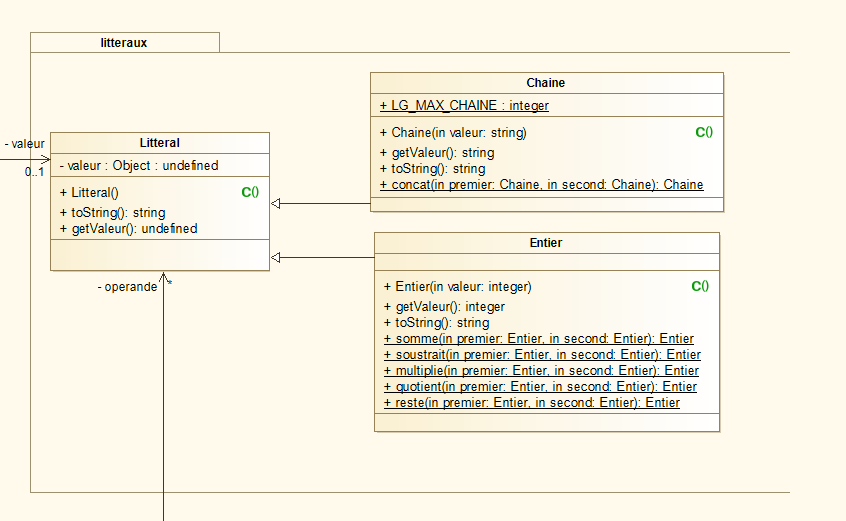
\includegraphics[scale=0.75]{./img/COO/COO_prototype_1/PackageLitteraux}\end{center}
\par Le choix de conception des littéraux a été une classe parente Litteral qui permet d'englober tous les types de données du programme.
La classe Entier a été détaillé dans la conception cependant elle n'a pas été codée à cette itération pour se concentrer sur les chaînes.
Les littéraux sont immuables pour permettre leur passage sans problème.

\section{Paquetage interpreteurlir.donnees}
\begin{center}\includegraphics[scale=0.65]{./img/COO/COO_prototype_1/PackageDonnees}\end{center}
\par Pour les données une classe variable a été choisie composée d'un littéral et d'un identificateur.
L'identificateur a comme classes dérivées les deux types affectables du projet soit les entiers et les chaînes.

\section{Paquetage interpreteurlir.expressions}
\begin{center}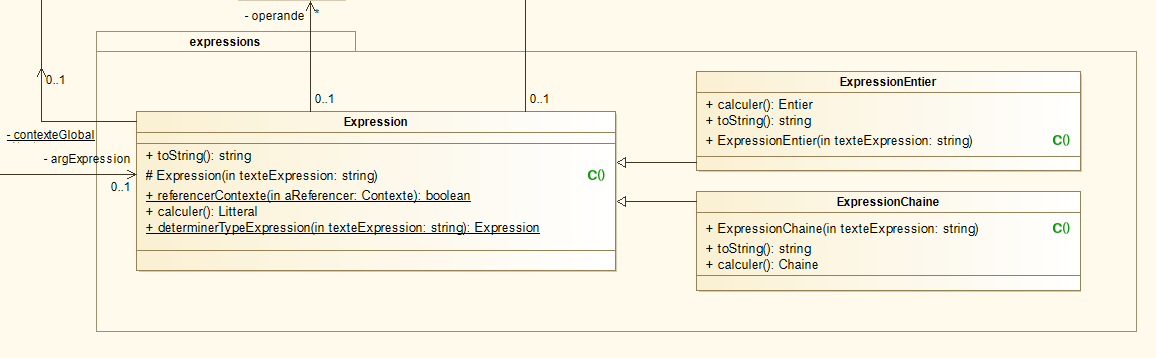
\includegraphics[scale=0.60]{./img/COO/COO_prototype_1/PackageExpressions}\end{center}
\par Comme pour le reste de notre conception les expressions sont typées et sont une spécialisation d'une classe Expression générale regroupant les comportements communs. Une méthode de classe d'Expression permet de créer le bon type d'expression.

\section{Paquetage interpreteurlir.motscles}
\begin{center}\includegraphics[scale=0.60]{./img/COO/COO_prototype_1/PackageMotscles}\end{center}
\par La conception de l'itération 1 contient ce qui devait être faits lors de cette itération à quelques détaille près comme la classe InstructionAffiche qui n'a pas été codée car non nécessaire aux fonctionnalités choisies.
L'itération 1 voulait permettre de manier des chaînes il fallait donc que les commandes connaissent le contexte contenant les variables. La solution choisie a été une attribut d'instance dans Commande initialiser à la construction de la commande par passage de la référence du contexte global par le constructeur. Une instance de commande correspond à un objet ayant toutes les informations nécessaire pour être exécuté (String arguments dans le constructeur). Les commandes et instructions fonctionnent en 2 temps, la construction qui valide les arguments et créer les éléments nécessaires à l'exécution puis l'exécution qui est la réalisation du comportement de la commande.

\section{Paquetage interpreteurlir}
\begin{center}\includegraphics[scale=0.60]{./img/COO/COO_prototype_1/PackageInterpreteurlir}\end{center}
\par Le contexte regroupe l'entièreté des variables définies dans la session courante. Une variable n'est accessible que par l'intermédiaire du contexte grâce à l'identificateur qui sert de clé. L'Analyseur est la classe qui permet le fonctionnement de tout. Une mainLoop permet de demander en continue une ligne à l'utilisateur puis celle-ci est analyser, à partir du mot clé une commande/instruction est crée en passant le reste de la ligne en argument. L'analyse des arguments se fait au niveau le plus interne possible (Analyseur analyse le mot cle, la commande les arguments qui construit ensuite les éléments dont elle a besoin qui s'occupe eux-mêmes de vérifier leur validité à la construction). Si une erreur dans la ligne à interprété est détecté alors une InterpreteurException est levée et se propage jusqu'à l'analyseur qui affiche l'erreur.

\section{Illustration avec des diagrammes d'objets}
\begin{center}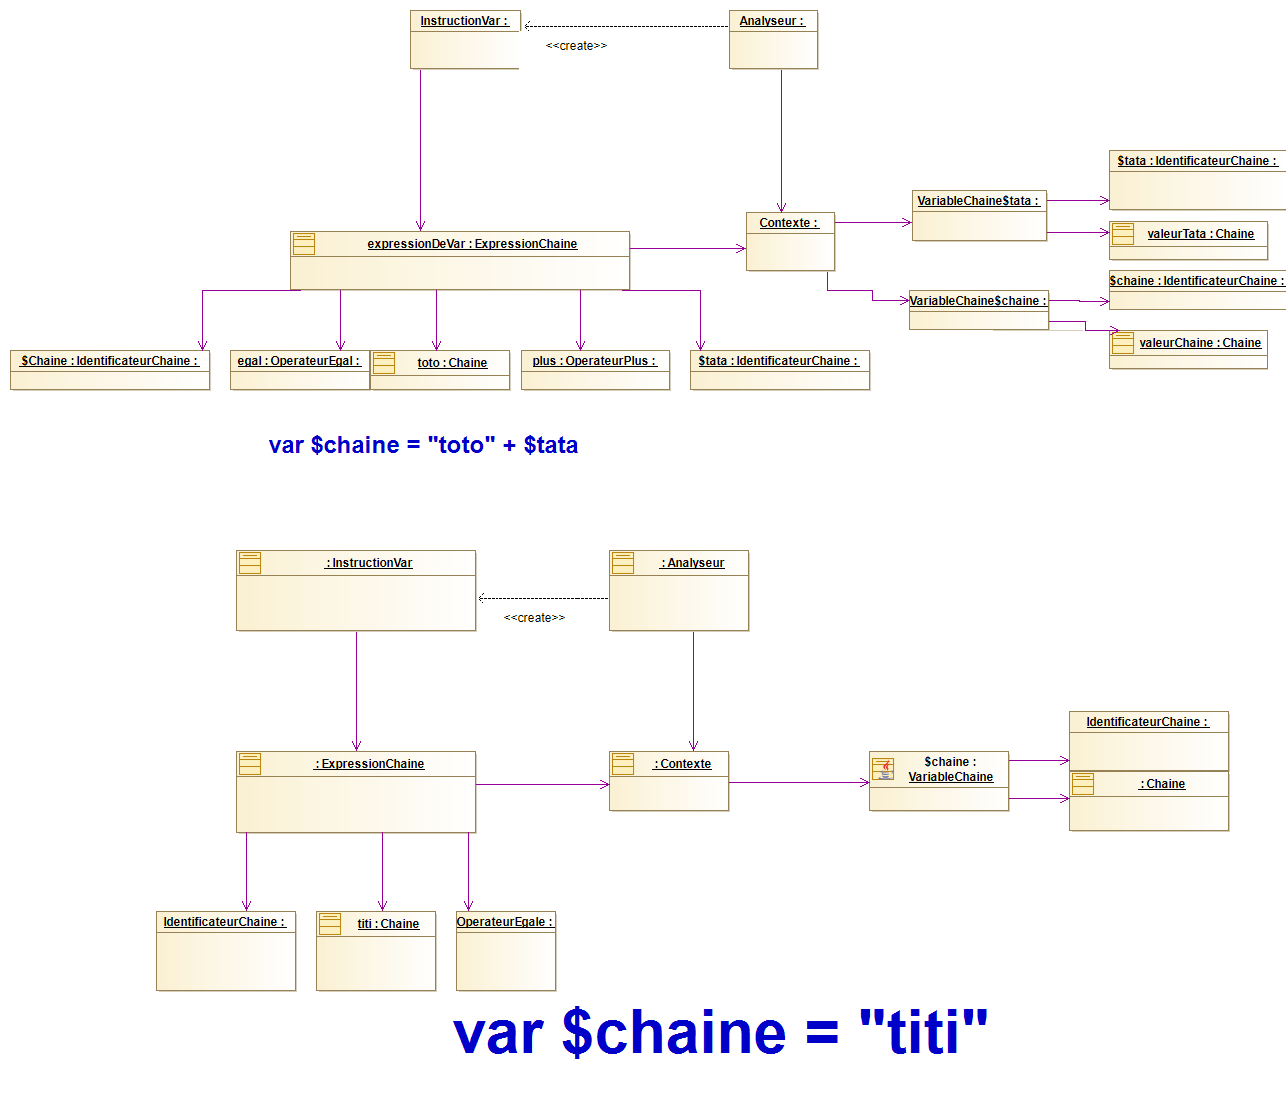
\includegraphics[scale=0.50]{./img/COO/COO_prototype_1/Objet}\end{center}
\par Voici des diagrammes qui ont été faits pendant la réflexion de cette conception. Ils permettent d'illustrer le fait qu'une instruction créer les éléments dont elle a besoin. Seul changement dans la conception par rapport à ces diagrammes : les opérateurs sont gérer en interne des instructions (il n'y pas de classe Operateur).

    \normalsize
    \chapter{Itération 2}

    \par L'itération 2 avait pour objectif d'ajouter le type entier. Puis il fallait pourvoir faire une programme, c'est-à-dire des instructions ordonnées avec des étiquettes exécutables plus tard. Pour compléter les objectifs de cette itération certaines commandes et instructions ont été réalisées (efface, liste, lance/affiche, entre, vaen, procedure, stop, retour).

\section{Diagrammes d'objets}
Comme conseillé par notre tuteur, nous avons commencé la conception de l'itération 2 par des diagrammes d'objets. Ci-dessous quelques exemples.
\par
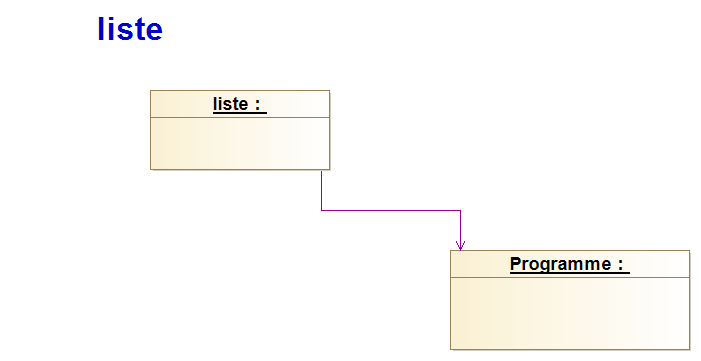
\includegraphics[scale=0.5]{./img/COO/COO_prototype_2/digrammesObjet/Diagramme d'objet la commande liste}
\par Le premier montre que la commande liste fait appel au programme (contenant les lignes de codes constituant un programmes) pour exécuter son comportement.
\par
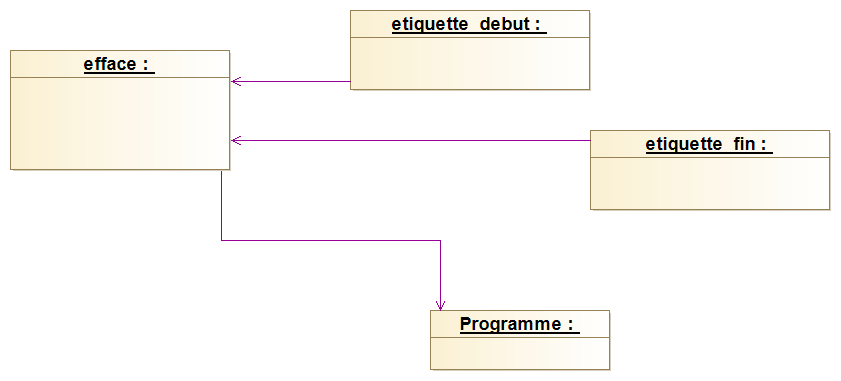
\includegraphics[scale=0.5]{./img/COO/COO_prototype_2/digrammesObjet/Diagramme d'objet de la commande efface}
\par La commande efface connait donc les deux étiquettes qui définissent sont comportement spécifique d'instance. Pour sont exécution elle doit connaitre le programme global de la session courante de l'interpréteur LIR.

\section{Paquetage interpreteurlir.donnees(.litteraux)}
\par Les paquetages donnees et litteraux n'ont que très peu changé en conception mais les classe liées aux entiers ont été codés pendant cette itération.

\section{Paquetage interpreteurlir.expressions}
\par Comme pour les données, pas de changement de conception mais programmtion de ExpressionEntier.

\section{Paquetage interpreteurlir.programmes}
\includegraphics[scale=0.5]{./img/COO/COO_prototype_2/PackageProgrammes}
\par Premièrement la classe étiquette permet d'ordonner les lignes de codes. Le Programme contient des méthodes pour tous les comportement qu'il doit réaliser ce qui permet de les intégrés en interne ce qui rend leur usage plus simple pour les commandes et instructions. Seul la méthode vaen est absente de la conception car nous nous sommes rendu compte qu'elle était nécessaire pendant la programmation. Autre changement, le programme doit enregistrés les lignes de codes. La conception montre une classe LigneCode prévue à cet effet cependant sur le conseil de notre tuteur nous avons utilisé une TreeMap<Etiquette, Instruction> ce qui a rendu LigneCode obsolète. La classe avait été programmée et testée mais nous l'avons supprimée car TreeMap était une meilleur solution.

\section{Paquetage interpreteurlir.motscles} 
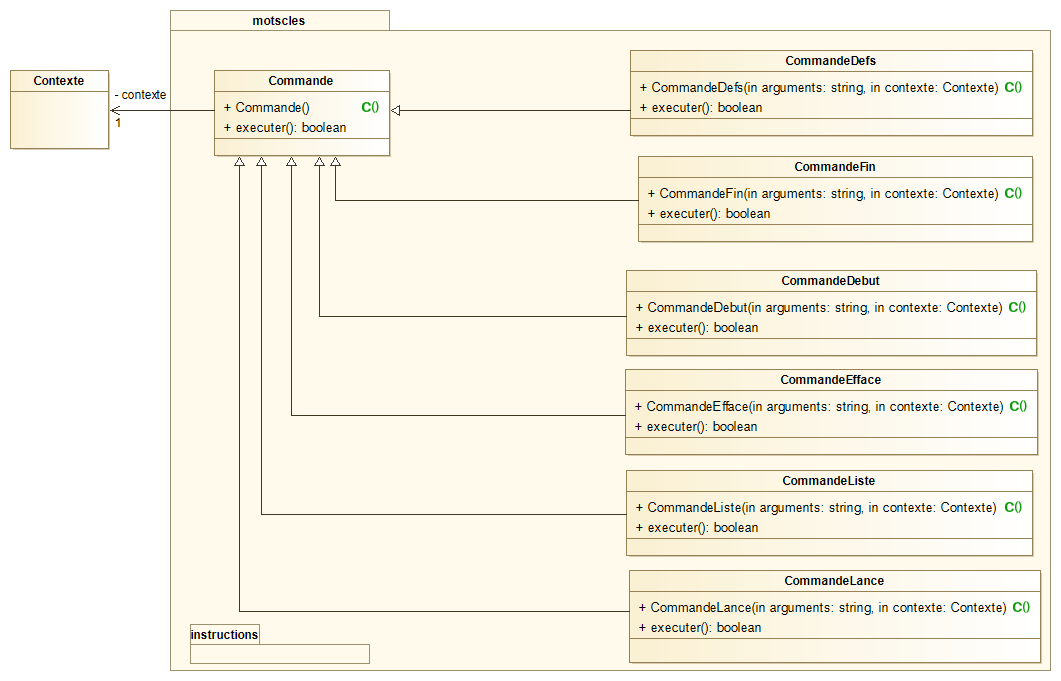
\includegraphics[scale=0.45]{./img/COO/COO_prototype_2/PackageCommande}
\par Les commandes à ajouter à cette itération ont été ajoutée à la conception en suivant le même principe de la dualité construction/exécution. Seul changement notable (non montré dans le diagramme car décidé pendant la programmation), l'ajout du programme nécessite que les commandes connaissent celui-ci. Après une longue réflexion nous avons choisis de le déclaré comme attribut protected dans la classe Commande et de le référencer au lancement de l'interpréteur sans savoir si c'était un bon choix ou non.

\section{Paquetage interpreteurlir.motscles.instructions} 
\includegraphics[scale=0.45]{./img/COO/COO_prototype_2/PackageInstruction}
\par Aucun changement notable, seulement ajout des nouvelles instructions.

\section{Paquetage interpreteurlir}
\includegraphics[scale=0.45]{./img/COO/COO_prototype_2/PackageInterpreteurlir}
\par Ajout de l'exception ExecutionException lancée pour une erreur à l'exécution comme une division par 0 (contrairement à l'InterpreteurException qui est lancée à la construction). Elle également affichée par l'Analyseur.

    \chapter{Itération 3}


    \par L'itération 3 à ajoutée les expressions booléennes avec l'instruction si vaen. Et les commandes permettent d'enregistrer et charger un programme LIR dans l'interpréteur (commande charge et sauve).

\section{Diagrammes d'objets}
\begin{center}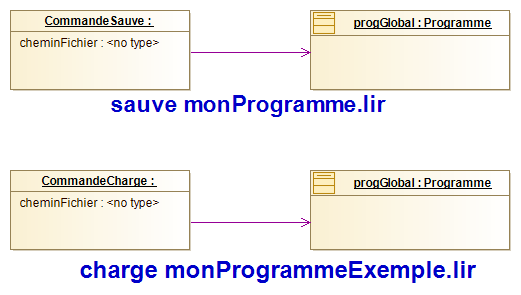
\includegraphics[scale=0.80]{fichiers/dossierPartieConception/img/COO/COO_prototype_3/digrammesObjet/charge}\end{center}
\par Les commandes sauve et charge sont liées au programme pour pouvoir charger ou récupérer des lignes de codes. Ces commandes connaissent une chaînes de texte correspondant au chemin du fichier.
\par
\begin{center}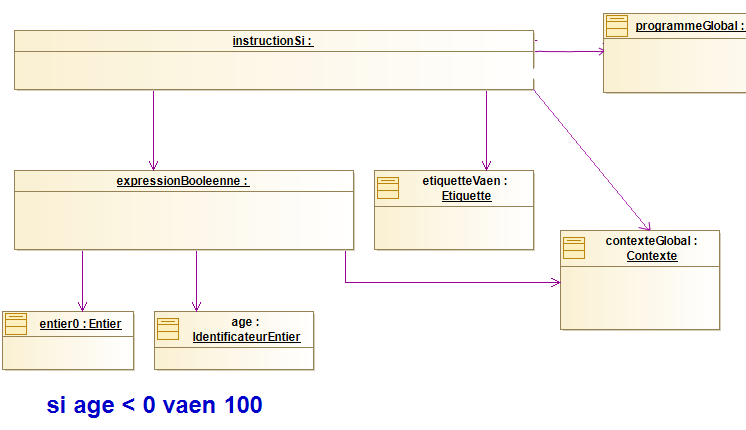
\includegraphics[scale=0.75]{fichiers/dossierPartieConception/img/COO/COO_prototype_3/digrammesObjet/siVaen}\end{center}
\par L'instruction si a besoin pour fonctionner d'une ExpressionBooleenne et de connaitre le contexte pour chercher les valeurs des variables à comparer. Elle doit connaitre l'étiquette où aller si la condition est vraie et donc du programme pour appeler la méthode du programme vaen.

\section{Paquetage interpreteurlir.donnees(.litteraux)}
\begin{center}\includegraphics[scale=0.40]{fichiers/dossierPartieConception/img/COO/COO_prototype_3/PackageDonnees}\end{center}
\par Le type booléen hérite de Litteral pour garder la logique de Litteral pouvant référencer chaque type de valeur du programme.

\section{Paquetage interpreteurlir.expressions}
\begin{center}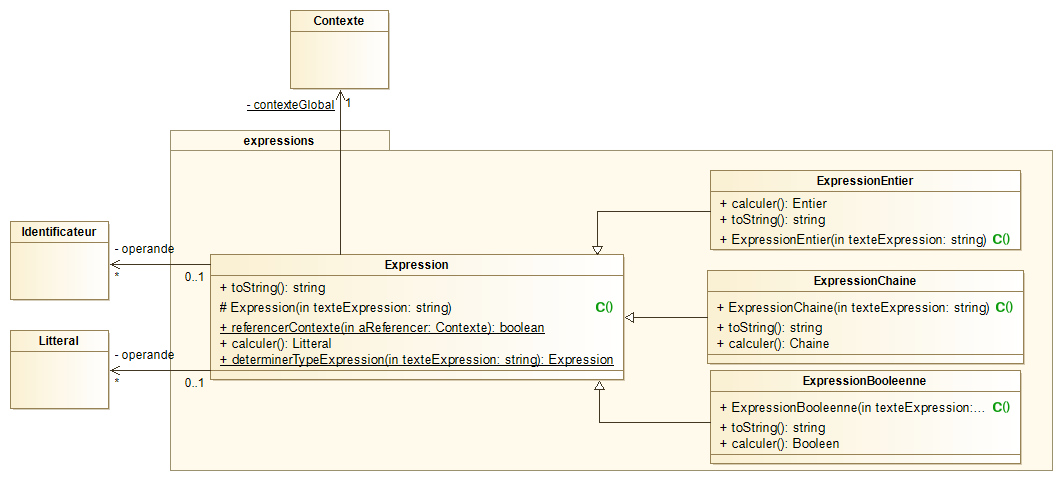
\includegraphics[scale=0.45]{fichiers/dossierPartieConception/img/COO/COO_prototype_3/PackageExpression}\end{center}
\par L'expression booléenne ne s'obtient pas avec la méthode determinerExpression car celle-ci est utilisée que par si vaen qui utilise que ce type d'expression. Le constructeur d'ExpressionBooleenne est donc utilisé directement.

\section{Diagramme de classes général}
\begin{center}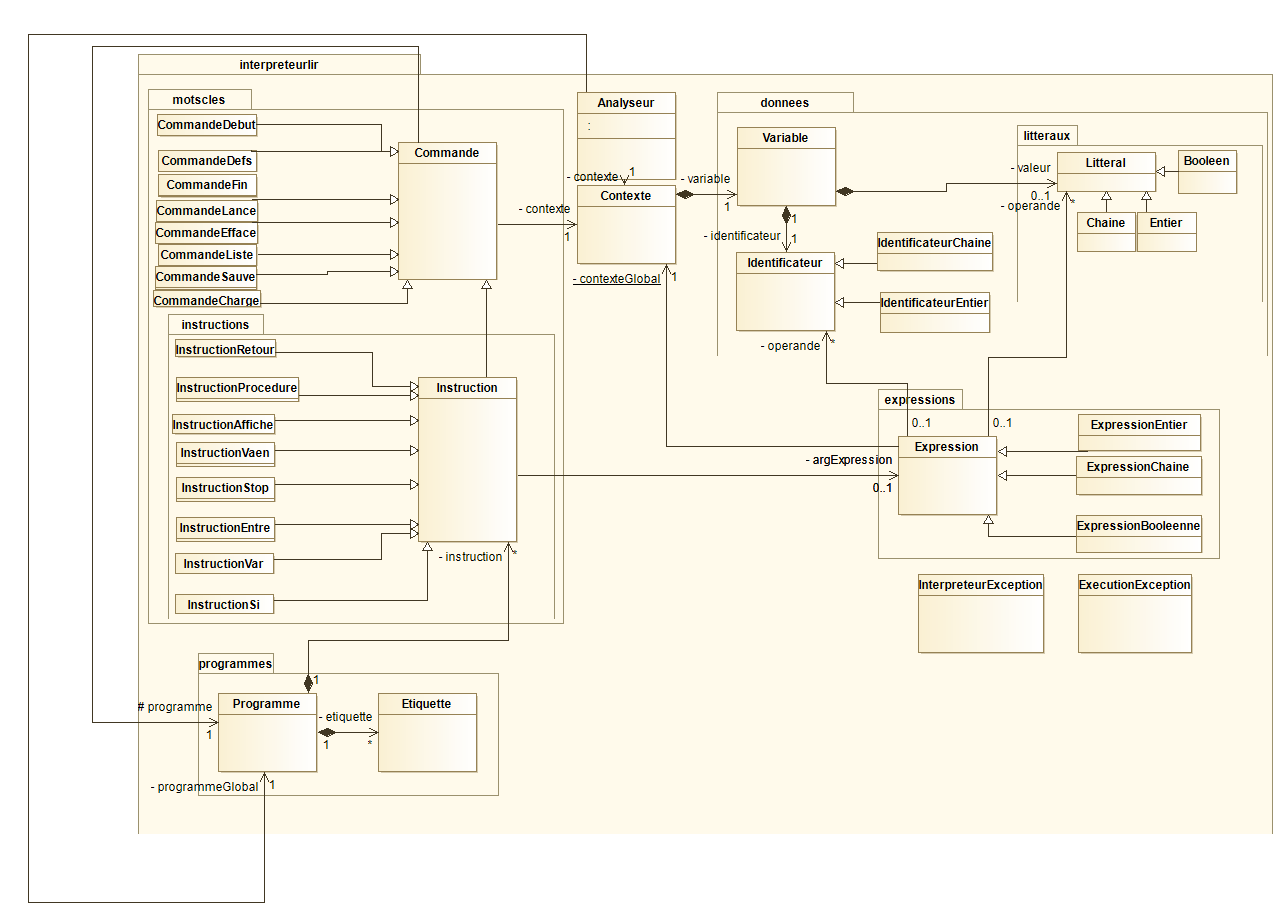
\includegraphics[scale=0.35]{fichiers/dossierPartieConception/img/COO/COO_prototype_3/Scéma général simplifié}\end{center}
\par Les commandes sauve et charge ont été ajoutés à la conception mais sont similaires aux autres commandes. Pareil pour l'instruction si vaen. Ce diagramme général permet de voir l'ensemble de la conception pour ce qui est des associations et généralisation des classes.

    \chapter{Projet final}

    \par Ce chapitre contient les diagrammes de classes représentant le logiciel codé. Les diagrammes de l'itération trois ont été complétés à partir du code pour ajouter les détails d'intégration dans le diagrammes (méthodes privées par exemple).

\section{Paquetage interpreteurlir.donnees(.litteraux)}
\begin{center}\includegraphics[scale=0.55]{./img/COO/PackageDonnees}\end{center}

\section{Paquetage interpreteurlir.expressions}
\begin{center}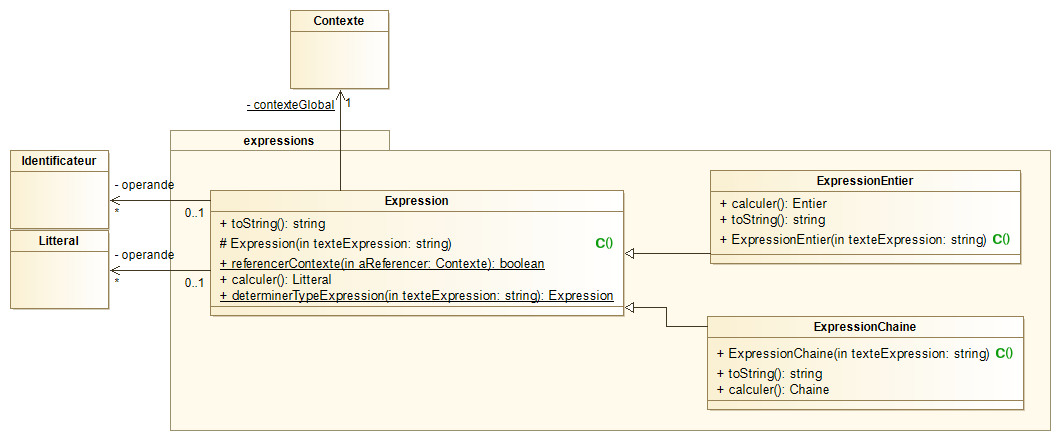
\includegraphics[scale=0.55]{./img/COO/PackageExpression}\end{center}

\section{Paquetage interpreteurlir.programmes}
\begin{center}\includegraphics[scale=0.55]{./img/COO/PackageProgrammes}\end{center}

\section{Paquetage interpreteurlir.motscles}
\begin{center}\includegraphics[scale=0.60]{./img/COO/PackageMotscles}\end{center}

\section{Paquetage interpreteurlir.motscles.instructions}
\begin{center}\includegraphics[scale=0.60]{./img/COO/PackageInstruction}\end{center}

\section{Paquetage interpreteurlir}
\begin{center}\includegraphics[scale=0.55]{./img/COO/PackageInterpreteurlir}\end{center}
    \part{Codage\\(annexe)}
%    \setcounter{chapter}{0}
    \part{Tests}
%    \setcounter{chapter}{0}
    \begin{enum}
    \item interpreteurlir.tests.TestContexte
\begin{verbatim}
    Exécution du test de Contexte#Contexte()
Réussite de testContexte
    Exécution du test de Contexte#raz()
Réussite de testRaz
    Exécution du test de Contexte#toString()
Réussite de testToString
    Exécution du test de Contexte#ajouterVariable(Identificateur, Litteral)
$chaine = "blabla"
$zoro = "Zoro le héro"
entier = 25

$abcd = "lol"
$chaine = "viveLa Vie"
$zoro = "   ah ah !  "
entier = -1

Réussite de testAjouterVariable
    Exécution du test de Contexte#lireValeurVariable(Identificateur)
Zoro le héro
Réussite de testLireValeurVariable
\end{verbatim}

    \item interpreteurlir.donnees.tests.TestIdentificateurChaine
\begin{verbatim}
    Exécution du test de IdentificateurEntier(String identificateur)
Réussite de testIdentificateurChaineString
    Exécution du test de getNom()
Réussite de testGetNom
\end{verbatim}

    \item interpreteurlir.donnees.tests.TestIdentificateurEntier
\begin{verbatim}
Réussite de testIdentificateurEntierString
Réussite de testGetNom
\end{verbatim}


    \item interpreteurlir.donnees.tests.TestVariable
\begin{verbatim}
    Exécution du test de toString()
Réussite de testToString
    Exécution du test de compareTo
Réussite de testCompareTo
    Exécution du test de Variable(Identificateur, Littéral)
Réussite de testVariableIdentificateurChaineLitteral
    Exécution du test de getIdentificateur()
Réussite de testGetIdentificateurChaine
    Exécution du test de getValeur()
Réussite de testGetValeurChaine
    Exécution du test de setValeur()
Réussite de testSetValeurChaine
\end{verbatim}

    \item interpreteurlir.donnees.litteraux.tests.TestBooleen
\begin{verbatim}
    Exécution du test de getValeur
Réussite de testGetValeur
\end{verbatim}

    \item interpreteurlir.donnees.litteraux.tests.TestChaine
\begin{verbatim}
    Exécution du test de Chaine(String)
Réussite de testChaine
    Exécution du test de toString
Réussite de testToString
    Exécution du test de compareTo(Chaine)
    Avec égalités
    Avec des inégalités
Réussite de testCompareTo
    Exécution du test de concaténer
Réussite de testConcatener
\end{verbatim}

    \item interpreteurlir.donnees.litteraux.tests.TestEntier
\begin{verbatim}
    Exécution du test de quotient(Entier, Entier) par 0
Réussite de testQuotientParZero
    Exécution du test de Entier(String)
Réussite de testEntierString
    Exécution du test de getValeur()
Réussite de testGetValeur
    Exécution du test de soustrait(Entier, Entier)
Réussite de testSoustrait
    Exécution du test de quotient(Entier, Entier)
Réussite de testQuotient
    Exécution du test de compareTo()
Réussite de testCompareTo
    Exécution du test de multiplie(Entier, Entier)
Réussite de testMultiplie
    Exécution du test de reste(Entier, Entier)
Réussite de testReste
    Exécution du test de Entier(String)
Réussite de testToString
    Exécution du test de somme(Entier, Entier)
Réussite de testSomme
    Exécution du test de reste(Entier, Entier) par 0
Réussite de testResteParZero
\end{verbatim}

    \item interpreteurlir.expression.tests.TestExpression
\begin{verbatim}
    Exécution du test de Expression#referencerContexte(Contexte)
Réussite de testReferencerContexte
    Exécution du test de Expression#determinerTypeExpression(String)
Réussite de testDeterminerTypeExpression
\end{verbatim}

    \item interpreteurlir.expression.tests.TestExpressionBooleenne
\begin{verbatim}
    Exécution du test de ExpressionBooleenne()
Réussite de testExpressionBooleenne
    Exécution du test de Calculer()
Réussite de testCalculer
    Exécution du test de toString()
Réussite de testToString
\end{verbatim}

    \item interpreteurlir.expression.tests.TestExpressionChaine
\begin{verbatim}
    Exécution du test de ExpressionChaine#ExpressionChaine(String)
Réussite de testExpressionChaineString
    Exécution du test de ExpressionChaine#calculer()
    Contexte initial : 
$toto = "valToto"

Calcul de : $chaine = "texte"
    Contexte : 
$chaine = "texte"
$toto = "valToto"


Calcul de : $chaine = "tata"
    Contexte : 
$chaine = "tata"
$toto = "valToto"


Calcul de : $tata
    Contexte : 
$chaine = "tata"
$toto = "valToto"


Calcul de : "une chaine de texte"
    Contexte : 
$chaine = "tata"
$toto = "valToto"


Calcul de : $chaine = "toto" + "titi"
    Contexte : 
$chaine = "tototiti"
$toto = "valToto"


Calcul de : $chaine = $toto + "titi"
    Contexte : 
$chaine = "valTototiti"
$toto = "valToto"


Calcul de : $chaine = "toto" + $titi
    Contexte : 
$chaine = "toto"
$toto = "valToto"


Calcul de : $chaine = $toto + $titi
    Contexte : 
$chaine = "valToto"
$toto = "valToto"


Calcul de : "toto" + "titi"
    Contexte : 
$chaine = "valToto"
$toto = "valToto"


Calcul de : $toto + "titi"
    Contexte : 
$chaine = "valToto"
$toto = "valToto"


Calcul de : "toto" + $titi
    Contexte : 
$chaine = "valToto"
$toto = "valToto"


Calcul de : $toto + $titi
    Contexte : 
$chaine = "valToto"
$toto = "valToto"


Calcul de : "ab=bc"
    Contexte : 
$chaine = "valToto"
$toto = "valToto"


Calcul de : $chaine = "ab+cd" + $toto
    Contexte : 
$chaine = "ab+cdvalToto"
$toto = "valToto"

Réussite de testCalculer
    Exécution du test de ExpressionChaine#toString()
Réussite de testToString
\end{verbatim}

    \item interpreteurlir.expression.tests.TestExpressionEntier
\begin{verbatim}
    Exécution du test de ExpressionEntier#calculer()
    Contexte initial : 
j34n = 1
marcel = 0
pi3rr3 = 2

Calcul de : entier = 2 + 3
    Contexte : 
entier = 5
j34n = 1
marcel = 0
pi3rr3 = 2


Calcul de : entier = 2 * 3
    Contexte : 
entier = 6
j34n = 1
marcel = 0
pi3rr3 = 2


Calcul de : bob = marcel - 2
    Contexte : 
bob = -2
entier = 6
j34n = 1
marcel = 0
pi3rr3 = 2


Calcul de : 45 + 14
    Contexte : 
bob = -2
entier = 6
j34n = 1
marcel = 0
pi3rr3 = 2


Calcul de : 45 * -2
    Contexte : 
bob = -2
entier = 6
j34n = 1
marcel = 0
pi3rr3 = 2


Calcul de : affectation = 64
    Contexte : 
affectation = 64
bob = -2
entier = 6
j34n = 1
marcel = 0
pi3rr3 = 2


Calcul de : affectation = marcel
    Contexte : 
affectation = 0
bob = -2
entier = 6
j34n = 1
marcel = 0
pi3rr3 = 2


Calcul de : entier = j34n + pi3rr3
    Contexte : 
affectation = 0
bob = -2
entier = 3
j34n = 1
marcel = 0
pi3rr3 = 2


Calcul de : entier = j34n
    Contexte : 
affectation = 0
bob = -2
entier = 1
j34n = 1
marcel = 0
pi3rr3 = 2


Calcul de : 42
    Contexte : 
affectation = 0
bob = -2
entier = 1
j34n = 1
marcel = 0
pi3rr3 = 2


Calcul de : rep0ns3 = 42
    Contexte : 
affectation = 0
bob = -2
entier = 1
j34n = 1
marcel = 0
pi3rr3 = 2
rep0ns3 = 42


Calcul de : division = 12 / 0
Attention Division par 0

Calcul de : modulo = 12 % 0
Attention Division par 0
Réussite de testCalculer
    Exécution du test de ExpressionEntier#toString()
Réussite de testToString
    Exécution du test de ExpressionEntier#ExpressionEntier(String)
Réussite de testExpressionEntierString
\end{verbatim}

    \item interpreteurlir.motscles.tests.TestCommandeCharge
\begin{verbatim}
Test valides de CommandeCharge#executer():
Test 1\7:
5 var $test = "fichier1 OK"
10 stop
Test 2\7:
5 var $test = "fichier2 OK"
10 stop
Test 3\7:
5 var $test = "fichier3 OK"
10 stop
Test 4\7:
5 var $test = "fichier4 OK"
10 stop
Test 5\7:
5 var $test = "fichier5 OK"
10 stop
Test 6\7:
5 var $test = "fichier6 OK"
10 stop
Test 7\7:
5 var $test = "fichier7 OK"
10 stop

Test invalides de CommandeCharge#executer():
aucune ligne à afficher
aucune ligne à afficher
Réussite de testExecuter
Réussite de testCommandeCharge
\end{verbatim}

    \item interpreteurlir.motscles.tests.TestCommandeDebut
\begin{verbatim}
    Exécution du test de CommandeDebut#executer()
Réussite de testExecuter
    Exécution du test de CommandeDebut#CommandeDebut(String, Contexte)
Réussite de testCommandeDebutStringContexte
\end{verbatim}

    \item interpreteurlir.motscles.tests.TestCommandeDefs
\begin{verbatim}
    Exécution du test de CommandeDefs#CommandeDefs(String, Contexte)
Réussite de testCommandeDefsStringContexte
    Exécution du test de CommandeDefs#executer()
Affichage du contexte :
aucune variable n'est définie
Affichage du contexte :
aucune variable n'est définie
Affichage du contexte :
aucune variable n'est définie
Réussite de testExecuter
\end{verbatim}

    \item interpreteurlir.motscles.tests.TestCommandeEfface
\begin{verbatim}
    Exécution du test de CommandeEfface(String, Contexte)
Réussite de testCommandeEfface
    Exécution du test d'executer()
Test visuel :
10 affiche Bonjour
20 affiche Comment
30 affiche Allez
40 affiche Vous
50 affiche foobar

10 affiche Bonjour
40 affiche Vous
50 affiche foobar

Réussite de testExecuter
\end{verbatim}

    \item interpreteurlir.motscles.tests.TestCommandeFin
\begin{verbatim}
    Exécution du test de CommandeFin#executer()
    Le programme doit s'éteindre en affichant un message d'aurevoir :
Test exécuter désactiver
Réussite de testExecuter
    Exécution du test de CommandeFin#CommandeFin(String, Contexte)
Réussite de testCommandeFinStringContexte
\end{verbatim}

    \item interpreteurlir.motscles.tests.TestCommandeLance
\begin{verbatim}
    Exécution du test de CommandeLance#executer()
Réussite de testExecuter
    Exécution du test de CommandeLance#CommandeLance(String, Contexte)
Réussite de testCommandeLance
\end{verbatim}

    \item interpreteurlir.motscles.tests.TestCommandeListe
\begin{verbatim}
    Exécution du test de CommandeListe#executer()
1 var $res = "1 "
10 var $res = $res + "10 "
13 var $res = $res + "13 "
25 var $res = $res + "25 "
31 var $res = $res + "31 "
40 var $res = $res + "40 "
78 var $res = $res + "78 "
89 var $res = $res + "89 "
13 var $res = $res + "13 "
25 var $res = $res + "25 "
25 var $res = $res + "25 "
31 var $res = $res + "31 "
40 var $res = $res + "40 "
40 var $res = $res + "40 "
78 var $res = $res + "78 "
89 var $res = $res + "89 "
Réussite de testExecuter
    Exécution du test de CommandeListe#CommandeListe(String, Contexte)
Réussite de testCommandeListe
\end{verbatim}

    \item interpreteurlir.motscles.tests.TestCommandeSauve
\begin{verbatim}
    Exécution du test de CommandeSauve#CommandeSauve(String, Contexte)
Réussite de testCommandeSauveStringContexte
    Exécution du test de CommandeSauve#executer()
Réussite de testExecuter
\end{verbatim}

    \item interpreteurlir.motscles.instructions.tests.TestInstructionAffiche
\begin{verbatim}
    Exécution du test de InstructionAffiche(String, Contexte)
Réussite de testInstructionAffiche
    Exécution du test de executer()
TEST VISUEL SUR CONSOLE :

    test visuel suivant : 


    test visuel suivant : 


    test visuel suivant : 
Hello World !!!
    test visuel suivant : 
6
    test visuel suivant : 
0
    test visuel suivant : 
-3
    test visuel suivant : 

    test visuel suivant : 
coucou
    test visuel suivant : 
300000000000000000 ça passe
Réussite de testExecuter
    Exécution du test de toString()
Réussite de testToString
\end{verbatim}

    \item interpreteurlir.motscles.instructions.tests.TestInstructionEntre
\begin{verbatim}
    Exécution du test de InstructionEntre#toString()
Réussite de testToString
Execution du test de InstructionEntre#executer()
? entre $chaine
"uneChaine"
ok
? entre $toto
"uneAutreChaine"
ok
? entre entier
42
ok
? entre resultat
10
ok
Contexte : 
$chaine = ""uneChaine""
$toto = ""uneAutreChaine""
entier = 42
resultat = 10

Réussite de testExecuter
    Exécution du test de InstructionEntre#InstructionEntre(String, Contexte)
Réussite de testInstructionEntreStringContexte
\end{verbatim}


    \item interpreteurlir.motscles.instructions.tests.TestInstructionProcedure
\begin{verbatim}
    Execution du test de InstructionProcedure#toString()
Réussite de testToString
    Execution du test de InstructionProcedure#executer()
Réussite de testExecuter
    Execution du test de InstructionProcedure#InstructionProcedure(String, Contexte)
Réussite de testInstructionProcedureStringContexte
\end{verbatim}

    \item interpreteurlir.motscles.instructions.tests.TestInstructionRetour
\begin{verbatim}
     Exécution du test de InstructionRetour#InstructionRetour(String, Contexte)
Réussite de testInstructionRetourStringContexte
    Execution du test de InstructionRetour#executer()
Réussite de testExecuter
    Execution du test de InstructionRetour#toString()
Réussite de testToString
\end{verbatim}

    \item interpreteurlir.motscles.instructions.tests.TestInstructionSi
\begin{verbatim}
    Exécution du test de InstructionSi#toString()
Réussite de testToString
    Exécution du test de InstructionSi#executer()
Réussite de testExecuter
    Exécution du test de InstructionSi#InstructionSi(String, Contexte)
Réussite de testInstructionSiStringContexte
\end{verbatim}

    \item interpreteurlir.motscles.instructions.tests.TestInstructionStop
\begin{verbatim}
    Exécution du test de executer()
Test Visuels

10 affiche "Bonjour"
20 affiche "Comment"
30 affiche "Allez"
40 affiche "Vous"
45 stop
50 affiche "foobar"

lancement du programme : ne doit pas afficher foobar
BonjourCommentAllezVous
Réussite de testExecuter
    Exécution du test de toString()
Réussite de testToString
    Exécution du test de InstructionStop(String, Contexte)
Réussite de testInstructionStop
\end{verbatim}

    \item interpreteurlir.motscles.instructions.tests.TestInstructionVaen
\begin{verbatim}
    Execution du test de InstructionVaen#InstructionVaen(String, Contexte)
Réussite de testInstructionVaenStringContexte
    Execution du test de InstructionVaen#executer()
Test visuel : Ne doit pas afficher les étiquettes (25, 31, 40 )
1 10 13 78 89 
Réussite de testExecuter
    Execution du test de InstructionVaen#toString()
Réussite de testToString
\end{verbatim}

    \item interpreteurlir.motscles.instructions.tests.TestInstructionVar
\begin{verbatim}
    Exécution du test de InstructionVar(String, Contexte)
Réussite de testInstructionVar
    Exécution du tes de toString()
Réussite de testToString
\end{verbatim}

    \item interpreteurlir.programmes.tests.TestEtiquette
\begin{verbatim}
    Exécution du test de Etiquette#Etiquette(int)
Réussite de testEtiquetteInt
    Exécution du test de Etiquette#Etiquette(String)
Réussite de testEtiquetteString
    Exécution du test de Etiquette#getValeur()
Réussite de testGetValeur
    Exécution du test de Etiquette#compareTo(Etiquette)
Réussite de testCompareTo
    Exécution du test de Etiquette#toString()
Réussite de testToString
\end{verbatim}

    \item interpreteurlir.programmes.tests.TestProgramme
\begin{verbatim}
    Exécution du test de Programme() : 
Réussite de testProgramme
    Exécution du test de toString() : 
Réussite de testToString
    Exécution du test de raz() : 
Réussite de testRaz
    Exécution du test de ajouterLigne() : 
Réussite de testAjouterLigne
    Exécution du test de listeBornee() : 
Réussite de testListeBornee
    Exécution du test de appelProcedure(Etiquette) : 
Réussite de testAppelProcedure
    Exécution du test de vaen(Etiquette) : voir TestInstructionVaen#testExecuter()
Réussite de testVaen
    Exécution du test de Programme#stop() : voir TestInstructionStop#testExecuter()
Réussite de testStop
    Exécution du test de lancer() TEST INTERACTIF : 
1 var $toto = "toto"
5 var $agreuagreu = "agreu"
10 var tata = 0 + 0
13 var $titi = "titi"
31 entre tutu
40 var entier = 93
89 var $youpi = "youpi lapin"

80
$agreuagreu = "agreu"
$titi = "titi"
$toto = "toto"
$youpi = "youpi lapin"
entier = 93
tata = 0
tutu = 80

Réussite de testLancer
    Exécution du test de effacer() : 
Réussite de testEffacer
    Exécution du test de retourProcedure() : 
Réussite de testRetourProcedure
    Exécution du test de lancer(Etiquette) TEST INTERACTIF : 
1 var $toto = "toto"
5 var $agreuagreu = "agreu"
10 var tata = 0 + 0
13 var $titi = "titi"
31 entre tutu
40 var entier = 93
89 var $youpi = "youpi lapin"

5
tutu = 5

10 var tata = 0 + 0
13 var $titi = "titi"
31 entre tutu
40 var entier = 93
89 var $youpi = "youpi lapin"

9
tutu = 9

31 entre tutu
40 var entier = 93
89 var $youpi = "youpi lapin"

10
tutu = 10

aucune ligne à afficher

aucune variable n'est définie

Réussite de testLancerEtiquette
\end{verbatim}
\end{enum}


    \part{Conclusion}
%    \setcounter{chapter}{0}
    \chapter{Conception et implémentation}

\section{Le livrable}

    \`{A} l'issue de ce projet, nous avons pu implémenter toutes les fonctionnalités de
    l'interpréteur LIR telles qu'elles étaient exposées dans le cahier des charges. Notre
    version de l'interpréteur fonctionne comme attendu par la MOA, bien que la gestion
    des erreurs et les messages affichés à l'écran auraient gagné à être plus précis et
    que certaines parties du code mériteraient une optimisation.

\section{Conception}

    Ce besoin d'optimisation découle de difficultés rencontrées lors de la conception des
    classes. Ces difficultés s'expliquent notamment par notre manque d'expérience. Si nous
    devions refaire ce projet, il est clair que certains des choix que nous avons faits ne
    seraient pas réitérés.

    Commencer directement par générer des diagrammes d'objets en lieu de diagrammes de
    classes nous aurait certainement permis de gagner quelques heures de travail au moment
    de la conception initiale. Nous avons cependant fait mieux pour intégrer des notions
    apprises au cours du projet, comme par exemple le passage en abstraction de certaines
    superclasses.

\chapter{Organisation du groupe}

    \section{Travail en binôme}

        Lors de chaque itération, nous avons autant que possible privilégié le travail
        en binôme, en fonction des disponibilités de chacun. Cette modalité nous a permis
        de nous assurer que tout le monde participait activement au développement et se
        sentait intégré et valorisé au sein du groupe.

        Nous avons aussi fait en sorte de mettre en place une rotation des binômes afin
        que chaque membre du groupe puisse travailler avec tout le monde. Nous avons ainsi
        pu nous confronter à d'autres de travailler, partager nos savoirs et nos
        expériences personnels et assurer une forte cohésion au sein du groupe.

    \section{Répartition de la charge de travail}

        Malheureusement, le travail en binôme n'est forcément garant d'une répartition
        efficace de la charge de travail. Cela pose en effet des contraintes cumulatives ;
        lorsque un membre du groupe a terminé sa tâche, si la suivante nécessite un travail
        à deux, ce membre devait parfois attendre que son binôme se libère. Il est arrivé
        qu'un des deux membres d'un binôme prenne du retard sur sa tâche. Cela a
        occasionnellement posé un frein sur cette modalité de travail.

        Devant travailler le weekend, nous nous sommes également heurtés aux aléas des
        disponibilités personnelles de chacun. Nous avons donc dû composer avec des
        contraintes familiales, universitaires (devoirs à rendre, révisions,...) ou
        personnelles. Ces difficultés seraient mitigées dans un contexte professionnel
        avec des horaires de travail définis dans un contrat.

        Nous regrettons aussi de ne pas avoir mis en place un roulement dans les
        responsabilités (chef de projet, secrétaire, gestionnaire de configuration). Nous
        avons préféré nous concentrer sur le code.

    \section{Communication}

        Tout au long du projet, nous avons mis l'accent sur la communication, afin
        de toujours avoir un aperçu de l'avancée de notre travail. L'utilisation d'un
        serveur \emph{Discord} dédié au projet a été un outil primordial. En effet,
        cet outil nous a permis de travailler en binôme en visioconférence, d'organiser
        des réunions MOE en distanciel.

        L'utilisation de \og{}salons \fg{} thématiques de
        conversation a aussi ouvert la possibilité de s'entraider lorsqu'une difficulté se
        présentait, faire circuler les informations, organiser les réunions, ou plus
        simplement discuter (moments de convivialité). Grâce à la synchronisation avec
        le dépôt Github, chaque membre recevait en temps réel les notifications sur
        l'évolution du projet.

        Nous pensons que la communication a été un atout de taille dans la conduite de
        ce projet. En effet, elle nous a permis de surmonter au mieux les difficultés qui
        se sont présentées au cours de la conception et du développement de l'interpréteur.

\chapter{Conclusion générale}

    Nous avons vécu ce projet comme une expérience enrichissante que nous considérons dans
    l'ensemble comme une réussite. Nous avons pu acquérir et consolider des compétences
    précieuses au travail d'équipe. Nous tâcherons au cours des prochains projets tutorés
    de réinvestir nos succès et apprendre de nos échecs.

    % Fin du corps de votre document .................................

    \appendix
    % Annexes jointes au dossier .....................................
    \part{Manuel utilisateur}

\end{document}